% Dmitry Mikushin, USI Lugano, dmitry.mikushin@usi.ch,
% using portions of original style file by Tom Cashman
%
% IMPORTANT NOTICE:
%
% The USI logo is unique; it is authorized for use only by employees of the
% Università della Svizzera italiana for work-related projects; others can use them
% ONLY with prior authorization (contact: press@usi.ch).
%
% http://www.press.usi.ch/en/corporate-design/corporate-design-stampa.htm
%
% This is an example beamer presentation, which uses Università della Svizzera italiana
% design theme.

\documentclass[aspectratio=169]{beamer}

% Packages
\usetheme{usi}
\usepackage{array}
\usepackage[backend=biber]{biblatex}
\usepackage{caption}
\usepackage{float}
\usepackage{graphicx}
\usepackage{hhline}
\usepackage{multirow}
\usepackage{pgfplots}
\usepackage{subcaption}
\usepackage{tikz}
\usepackage{xcolor}


\colorlet{punct}{red!60!black}
\definecolor{background}{HTML}{EEEEEE}
\definecolor{delim}{RGB}{20,105,176}
\colorlet{numb}{magenta!60!black}
\usepackage{listings}
\lstdefinelanguage{json}{
    basicstyle=\normalfont\ttfamily,
    numbers=left,
    numberstyle=\footnotesize,
    stepnumber=1,
    numbersep=8pt,
    showstringspaces=false,
    breaklines=true,
    frame=lines,
    backgroundcolor=\color{background},
    literate=
     *{0}{{{\color{numb}0}}}{1}
      {1}{{{\color{numb}1}}}{1}
      {2}{{{\color{numb}2}}}{1}
      {3}{{{\color{numb}3}}}{1}
      {4}{{{\color{numb}4}}}{1}
      {5}{{{\color{numb}5}}}{1}
      {6}{{{\color{numb}6}}}{1}
      {7}{{{\color{numb}7}}}{1}
      {8}{{{\color{numb}8}}}{1}
      {9}{{{\color{numb}9}}}{1}
      {:}{{{\color{punct}{:}}}}{1}
      {,}{{{\color{punct}{,}}}}{1}
      {\{}{{{\color{delim}{\{}}}}{1}
      {\}}{{{\color{delim}{\}}}}}{1}
      {[}{{{\color{delim}{[}}}}{1}
      {]}{{{\color{delim}{]}}}}{1},
}

% Bibliography source.
\addbibresource{references.bib}

% Colour definitions
\definecolor{mycolor3}{RGB}{170,35,3}

\setlength{\fboxsep}{0.25pt}
\setlength{\fboxrule}{0pt}

\title[Particle Simulations with OpenACC]{\textbf{Evaluating large scale particle simulations with OpenACC}\\[0.5em] Status Update}
\author{Samuel A. Cruz Alegr\'{i}a, Alessandra M. de Felice, Hrishikesh R. Gupta}
\institute{(University of Lugano)}
\date{\today}


\begin{document}
%-------------------------------------------------------------------------------	
\begin{frame}
\titlepage
\end{frame}
%-------------------------------------------------------------------------------

%-------------------------------------------------------------------------------
\begin{frame}[fragile]{Accomplishments thus far}

Our accomplishments thus far include the following:
%
\begin{itemize}
	\item Encoding particle movement in three dimensions.
	\item Using ParaView for visualizing our results.
	\item Including OpenACC parallel loops in the code.
\end{itemize}
%
Furthermore, an attempt has been made at simulating realistic particle interactions.

\end{frame}
%-------------------------------------------------------------------------------

%-------------------------------------------------------------------------------
\begin{frame}[fragile]{Serial code}
	The code mainly performs the following tasks:
	%
	\begin{enumerate}
		\item Initializing particle positions.
		\item Updating particle details such as position and velocity.
		\item Writing particle details to a file in every time step.
	\end{enumerate}
	%
\end{frame}
%-------------------------------------------------------------------------------

%-------------------------------------------------------------------------------
\begin{frame}[fragile]{Serial code}
	Demo at the end...
\end{frame}
%-------------------------------------------------------------------------------

%-------------------------------------------------------------------------------
\begin{frame}[fragile]{Visualization tools}
	In order to facilitate visualization of the particle simulation, we have decided to use \emph{ParaView}. 
\end{frame}
%-------------------------------------------------------------------------------

%-------------------------------------------------------------------------------
\begin{frame}[fragile]{Visualization tools}
	\emph{ParaView} \cite{website:paraview_wiki}.
	%
	\begin{itemize}
		\item Used at the CSCS (Swiss National Supercomputing Centre) \cite{website:cscs}.
		\item Open source, used for visualizing two and three-dimensional data sets.
		\item Platforms supported range from single-processor workstations to multiple-processor distributed-memory supercomputers or workstation clusters.
		\item Many file formats supported.
	\end{itemize}
	%
\end{frame}
%-------------------------------------------------------------------------------

%-------------------------------------------------------------------------------
\begin{frame}[fragile]{Visualization tools}
	We are using the VTK file format, which consists of the following header
	%
	\begin{lstlisting}[language=json]
	# vtk DataFile Version 1.0
	3D triangulation data
	ASCII

	DATASET POLYDATA
	POINTS N float
	\end{lstlisting}
	%
	and the following body
	%
	\begin{table}
		\centering
		\begin{tabular}{l l l}
			\emph{x-coordinate} & \emph{y-coordinate} & \emph{z-coordinate} \\
			$p0_x$ & $p0_y$ & $p0_z$\\
			\vdots & \vdots & \vdots\\
			$pN_x$ & $pN_y$ & $pN_z$\\
		\end{tabular}
	\end{table}
	%
\end{frame}
%-------------------------------------------------------------------------------

%-------------------------------------------------------------------------------
\begin{frame}[fragile]{Visualization tools}
	Using the VTK file format, we create a file for each time step. In each file, we write the position of each particle in the given time step.
	%
	\begin{itemize}
		\item \texttt{positions\_0.txt}
		\item \texttt{positions\_1.txt}
		\item \texttt{positions\_2.txt}
		\item And so on...
	\end{itemize}
	%
\end{frame}
%-------------------------------------------------------------------------------

%-------------------------------------------------------------------------------
\begin{frame}[fragile]{Parallelization methods}
	Preliminary benchmarks made for comparing execution time of \texttt{update\_particles()} function using serial version and parallel version (OpenACC).
\end{frame}
%-------------------------------------------------------------------------------

%-------------------------------------------------------------------------------
\begin{frame}[fragile]{Parallelization methods}
	% Performance comparison
	\begin{figure}[H]
		\centering
		%
\begin{tikzpicture}

% f(x)
\begin{axis}[
width=0.4\linewidth,
at={(0.0in,0.0in)},
separate axis lines,
every outer x axis line/.append style={black},
every x tick label/.append style={font=\footnotesize},
every outer y axis line/.append style={black},
every y tick label/.append style={font=\footnotesize},
xtick pos=left,
ytick pos=left,
xticklabel style={font=\footnotesize},
yticklabel style={font=\footnotesize},
yminorticks=true,
xmin=1000,
xmax=4000,
ymin=0,
ymax=400,
xlabel={Matrix size $n$},
ylabel={Execution time (seconds)},
label style={font=\footnotesize},
axis background/.style={fill=none},
legend style={at={(0,0)},legend cell align=left,align=left,draw=none,fill=none,font=\footnotesize},
legend entries={Serial,
                OpenACC},
legend pos=north west
]

\addlegendimage{black}
\addlegendimage{mycolor3}

\addplot+[color=black, line width=1.5pt,mark size=1.0pt,mark=none,mark options={fill=black}]
table[x=matrix_size,y=naive]{./Graphics/data/performance_comparison.txt}; \label{plot:avg_time_per_iter}

\addplot+[color=mycolor3, line width=1.5pt,mark size=1.0pt,mark=none,mark options={fill=mycolor3}]
table[x=matrix_size,y=openacc]{./Graphics/data/performance_comparison.txt};
\end{axis}
%

\end{tikzpicture}
%

		\caption{Matrix--matrix multiplication: execution time comparison.}
	\end{figure}
	%
\end{frame}
%-------------------------------------------------------------------------------

%-------------------------------------------------------------------------------
\begin{frame}[fragile]{Benchmarks}
% Performance comparison
\begin{center}
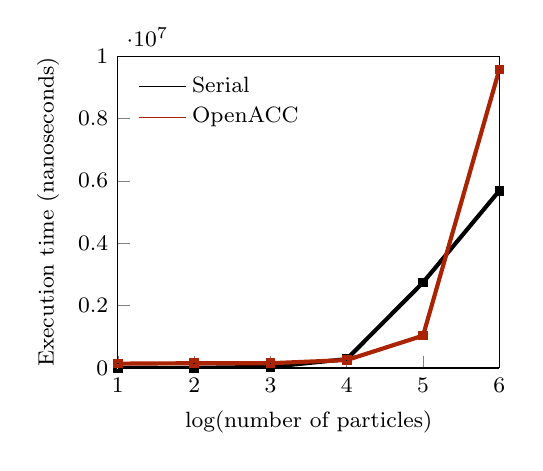
\begin{tikzpicture}

% f(x)
\begin{axis}[
width=0.53\linewidth,
at={(0.0in,0.0in)},
separate axis lines,
every outer x axis line/.append style={black},
every x tick label/.append style={font=\footnotesize},
every outer y axis line/.append style={black},
every y tick label/.append style={font=\footnotesize},
xtick pos=left,
ytick pos=left,
xticklabel style={font=\footnotesize},
yticklabel style={font=\footnotesize},
yminorticks=true,
xmin=1,
xmax=6,
ymin=0,
ymax=10000000,
xlabel={log(number of particles)},
xtick={1,2,3,4,5,6},
ylabel={Execution time (nanoseconds)},
label style={font=\footnotesize},
axis background/.style={fill=none},
legend style={at={(0,0)},legend cell align=left,align=left,draw=none,fill=none,font=\footnotesize},
legend entries={Serial,
	OpenACC},
legend pos=north west
]

\addlegendimage{black}
\addlegendimage{mycolor3}

\addplot[
color=black, line width=1.5pt,mark size=1.0pt,mark=square
]
coordinates {
(1,1241.21)(2,4739.75)(3,36627.6)(4,284549)(5,2742173)(6,5685342)
};
\addplot[
color=mycolor3, line width=1.5pt,mark size=1.0pt,mark=square
]
coordinates {
(1,139925)(2,153380)(3,153689 )(4,255065 )(5,1037473)(6,9572726)
};

\end{axis}
%

\end{tikzpicture}\\
\end{center}
%
\end{frame}
%-------------------------------------------------------------------------------

%-------------------------------------------------------------------------------
\begin{frame}[fragile]{Project plan}
	Show current project calendar...
\end{frame}
%-------------------------------------------------------------------------------

%-------------------------------------------------------------------------------
\begin{frame}[fragile]{References}
	\printbibliography
\end{frame}
%-------------------------------------------------------------------------------

%-------------------------------------------------------------------------------
\begin{frame}[fragile]{Questions}
	%
	\begin{center}
		Thank you for your attention!\\
		\\
		Any questions?
	\end{center}
	%
\end{frame}
%-------------------------------------------------------------------------------


\end{document}
